\section{System Model}
\label{sec:model}

\subsection{Field water balance}

This paper reuses, unchanged, the standardised root-zone water balance of FAO-56
chapter~8~\cite{fao56}, so that every auditor starts from the same point. The root-zone
water content $w_t$ [mm] evolves hourly under the bucket equation:
\begin{equation}
w_{t+1}=\mathrm{clip}_{\le FC}\!\left(w_t+P_t-RO_t-ET_{c,t}+u_t\right),
\label{eq:bucket}
\end{equation}
That is, water in minus water out, with any excess above field capacity clipped
away. Here:
\begin{symbolist}
\item[$w_t$] root-zone water content at hour $t$, in mm;
\item[$P_t$] rainfall during hour $t$, in mm;
\item[$RO_t$] surface runoff leaving the field during hour $t$, in mm, obtained
  from the curve-number method of the Soil Conservation Service (SCS-CN) published
  in 1972, evaluated daily and shared pro rata over the hours of a rain event;
\item[$ET_{c,t}$] crop evapotranspiration during hour $t$, in mm;
\item[$u_t$] irrigation depth applied in hour $t$, in mm, the only term supplied
  by the farmer's log;
\item[$FC$] field capacity, the largest water content the soil retains after free
  drainage, in mm;
\item[$\mathrm{clip}_{\le FC}$] the clipping operator, which passes values at or
  below $FC$ unchanged and maps anything above it to $FC$.
\end{symbolist}

$ET_{c,t}$ cannot be measured, so it is computed from reference
evapotranspiration by FAO-56 equations~83 and~84:
\begin{equation}
ET_{c,t}=K_{s,t}\,K_c\,ET_{0,t},
\qquad
K_{s,t}=\frac{FC-w_t}{(1-p)\,\mathrm{TAW}},
\label{eq:etc}
\end{equation}
where:
\begin{symbolist}
\item[$ET_{0,t}$] hourly reference evapotranspiration, computed by the hourly form
  of Penman-Monteith, FAO-56 equation~53, from public weather data;
\item[$K_c$] the crop coefficient, characterising how much water rice uses relative
  to the reference grass;
\item[$K_{s,t}$] the water-stress coefficient, falling from 1 towards 0 as the
  field dries, by FAO-56 equation~84;
\item[$p$] the fraction of available water the crop can still use before stress
  begins, taken from FAO-56;
\item[$\mathrm{TAW}$] total available water in the root zone, equal to $FC-WP$ by
  FAO-56 equation~82.
\end{symbolist} Drainage above field capacity $FC$ is removed by the clipping operator, so mass
conservation holds exactly and is checked as an invariant.

What decides a dry phase is the relative depletion of the root zone, normalised to the
interval from 0 to 1:
\begin{equation}
d_t=\frac{FC-w_t}{FC-WP},\qquad \mathrm{span}=FC-WP,
\label{eq:depl}
\end{equation}
where:
\begin{symbolist}
\item[$d_t$] root-zone depletion at hour $t$, a dimensionless fraction equal to 0 at
  field capacity and to 1 at the wilting point;
\item[$WP$] the wilting point, the moisture below which the crop can no longer
  extract water, in mm;
\item[$\mathrm{span}$] the width of the depletion scale, equal to $FC-WP$, used to
  convert the fraction $d_t$ into a water amount in mm.
\end{symbolist}

For the reference silty clay loam of the delta, the values
$\mathrm{TAW}=FC-WP=70$\,mm, $FC=160$\,mm, $WP=90$\,mm are the mid-range entries
of FAO-56 Table~12 for a $0.5$\,m root zone~\cite{fao56}. These three equations are
the whole physical basis the audit layer uses; no parameter is invented by us.

\subsection{Replay of a claimed log}
\label{sec:replay}

Let a claimed log supply the irrigation term of \eqref{eq:bucket}. The \emph{replay operator} $\mathcal{R}$ maps a log to the trajectory it implies. The
procedure substitutes the depths the farmer recorded into the $u_t$ slot of
\eqref{eq:bucket}, then iterates that equation hour by hour under the observed
forcing $(P_t,ET_{0,t})$:
\begin{equation}
\mathcal{R}(L)=\{(\hat w_t,\hat d_t)\}_{t=0}^{T},
\label{eq:replay}
\end{equation}
with $\hat w_0=w_{\mathrm{init}}$ and
\begin{equation}
u_t=\sum_{(t_i,u_i)\in L}u_i\,\mathbb{1}[t_i=t],
\label{eq:uterm}
\end{equation}
where:
\begin{symbolist}
\item[$L$] the claimed log, a list of hour-and-depth pairs recorded by the farmer;
\item[$T$] the total number of hours in the simulation window;
\item[$\hat w_t$] root-zone water content implied by the log, that is, the water the
  log \emph{claims} the field had at hour $t$;
\item[$\hat d_t$] the corresponding depletion fraction, obtained from $\hat w_t$
  through \eqref{eq:depl};
\item[$\hat w_0=w_{\mathrm{init}}$] the initial condition, the field's moisture
  state before the first irrigation;
\\item[{\\(\\mathbb{1}[\\cdot]\\)}] the indicator function, equal to 1 when the bracketed condition holds and 0
  otherwise.
\end{symbolist}

The hat marks quantities reconstructed from the log rather than measured. This is the
pivot of the whole paper: a replayed trajectory is what the farmer \emph{declared},
not what the field produced. Replay is
deterministic and uses only public reanalysis, so two auditors replaying the
same log obtain the same trajectory and the verdict is reproducible. Fig.~\ref{fig:method} summarises that path, from the farmer's log through the twin to the verdict of each defence tier. A
superscript minus denotes the state immediately \emph{before} that hour's
claim is applied, as in $\hat w_{t}^{-}$: the water available to receive an
event, which is what a filter must inspect.

The operator is also what makes the scheme cheap: no sensor is queried, and the
only inputs are the log, the public weather series and a soil profile. Its
weakness, developed in Sec.~\ref{sec:timeshift}, is that it can only check
whether a trajectory is \emph{possible}, never whether it \emph{happened}.


\begin{figure}[!t]
\centering
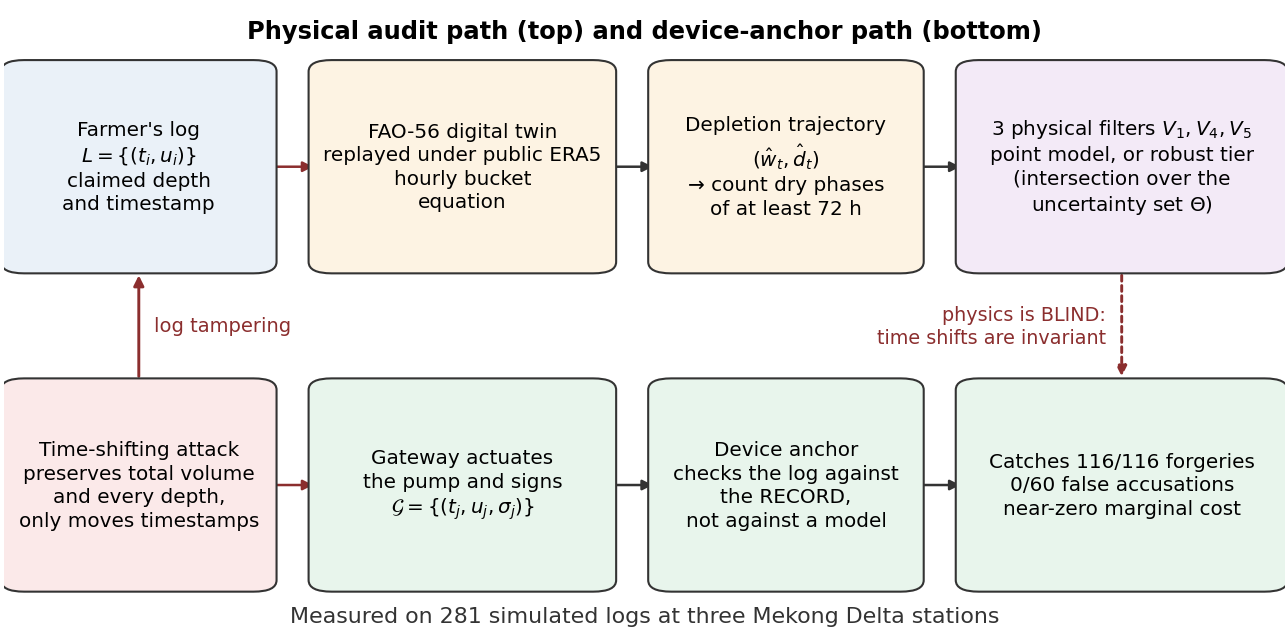
\includegraphics[height=6.9cm]{figures_vi/fig1_method_en.png}
\caption{Data flow of the method. The physical audit layer replays the claimed log through the water-balance twin and then through three filters; the device anchor checks the same log against the signed command record of the gateway. The dashed arrow shows the time-shifting attack passing through the physical layer undetected.}\label{fig:method}
\end{figure}
